\section{PI og PID koefficienter}
Bestemmelsen tager udgangspunkt i en analytisk fremgangsmåde ved brug af \emph{pidtool()} og Simulink simuleringen\footnote{Findes på CDROM.} af PTS. "Start" koefficienterne, angivet i tabel \ref{tb:PID_test14}.
\begin{figure}[h!]
\centering
\begin{tabu}{l|[1.25pt]c|c|c}
      & \(K_P\) & \(K_I\) & \(K_D\)\\\tabucline[1.25pt]{-}
Tilt  & 38,5 & 20 & -\\\hline%0,248960\\\hline
Pan   & 27 &  6,83 & -
\end{tabu}
\captionsetup{type=table}
\caption[Regulator koefficienter brugt i test]{Regulator koefficienter brugt til test af PTS.}
\label{tb:PID_test14} 
\end{figure}

Efter bestemmelsen af koefficienterne, blev de testet i controlleren. 
For at finde ud af, hvorgodt PTS med nævnte koefficienter lever op kravene for PTS, eksporteres den ønsket og aktuelle værdi for hhv. pan og tilt. Herefter blev den samlet difference for pan og tilt plottet i figur \ref{fig:PID_test14_plot}.
\begin{figure}[h!]
\centering
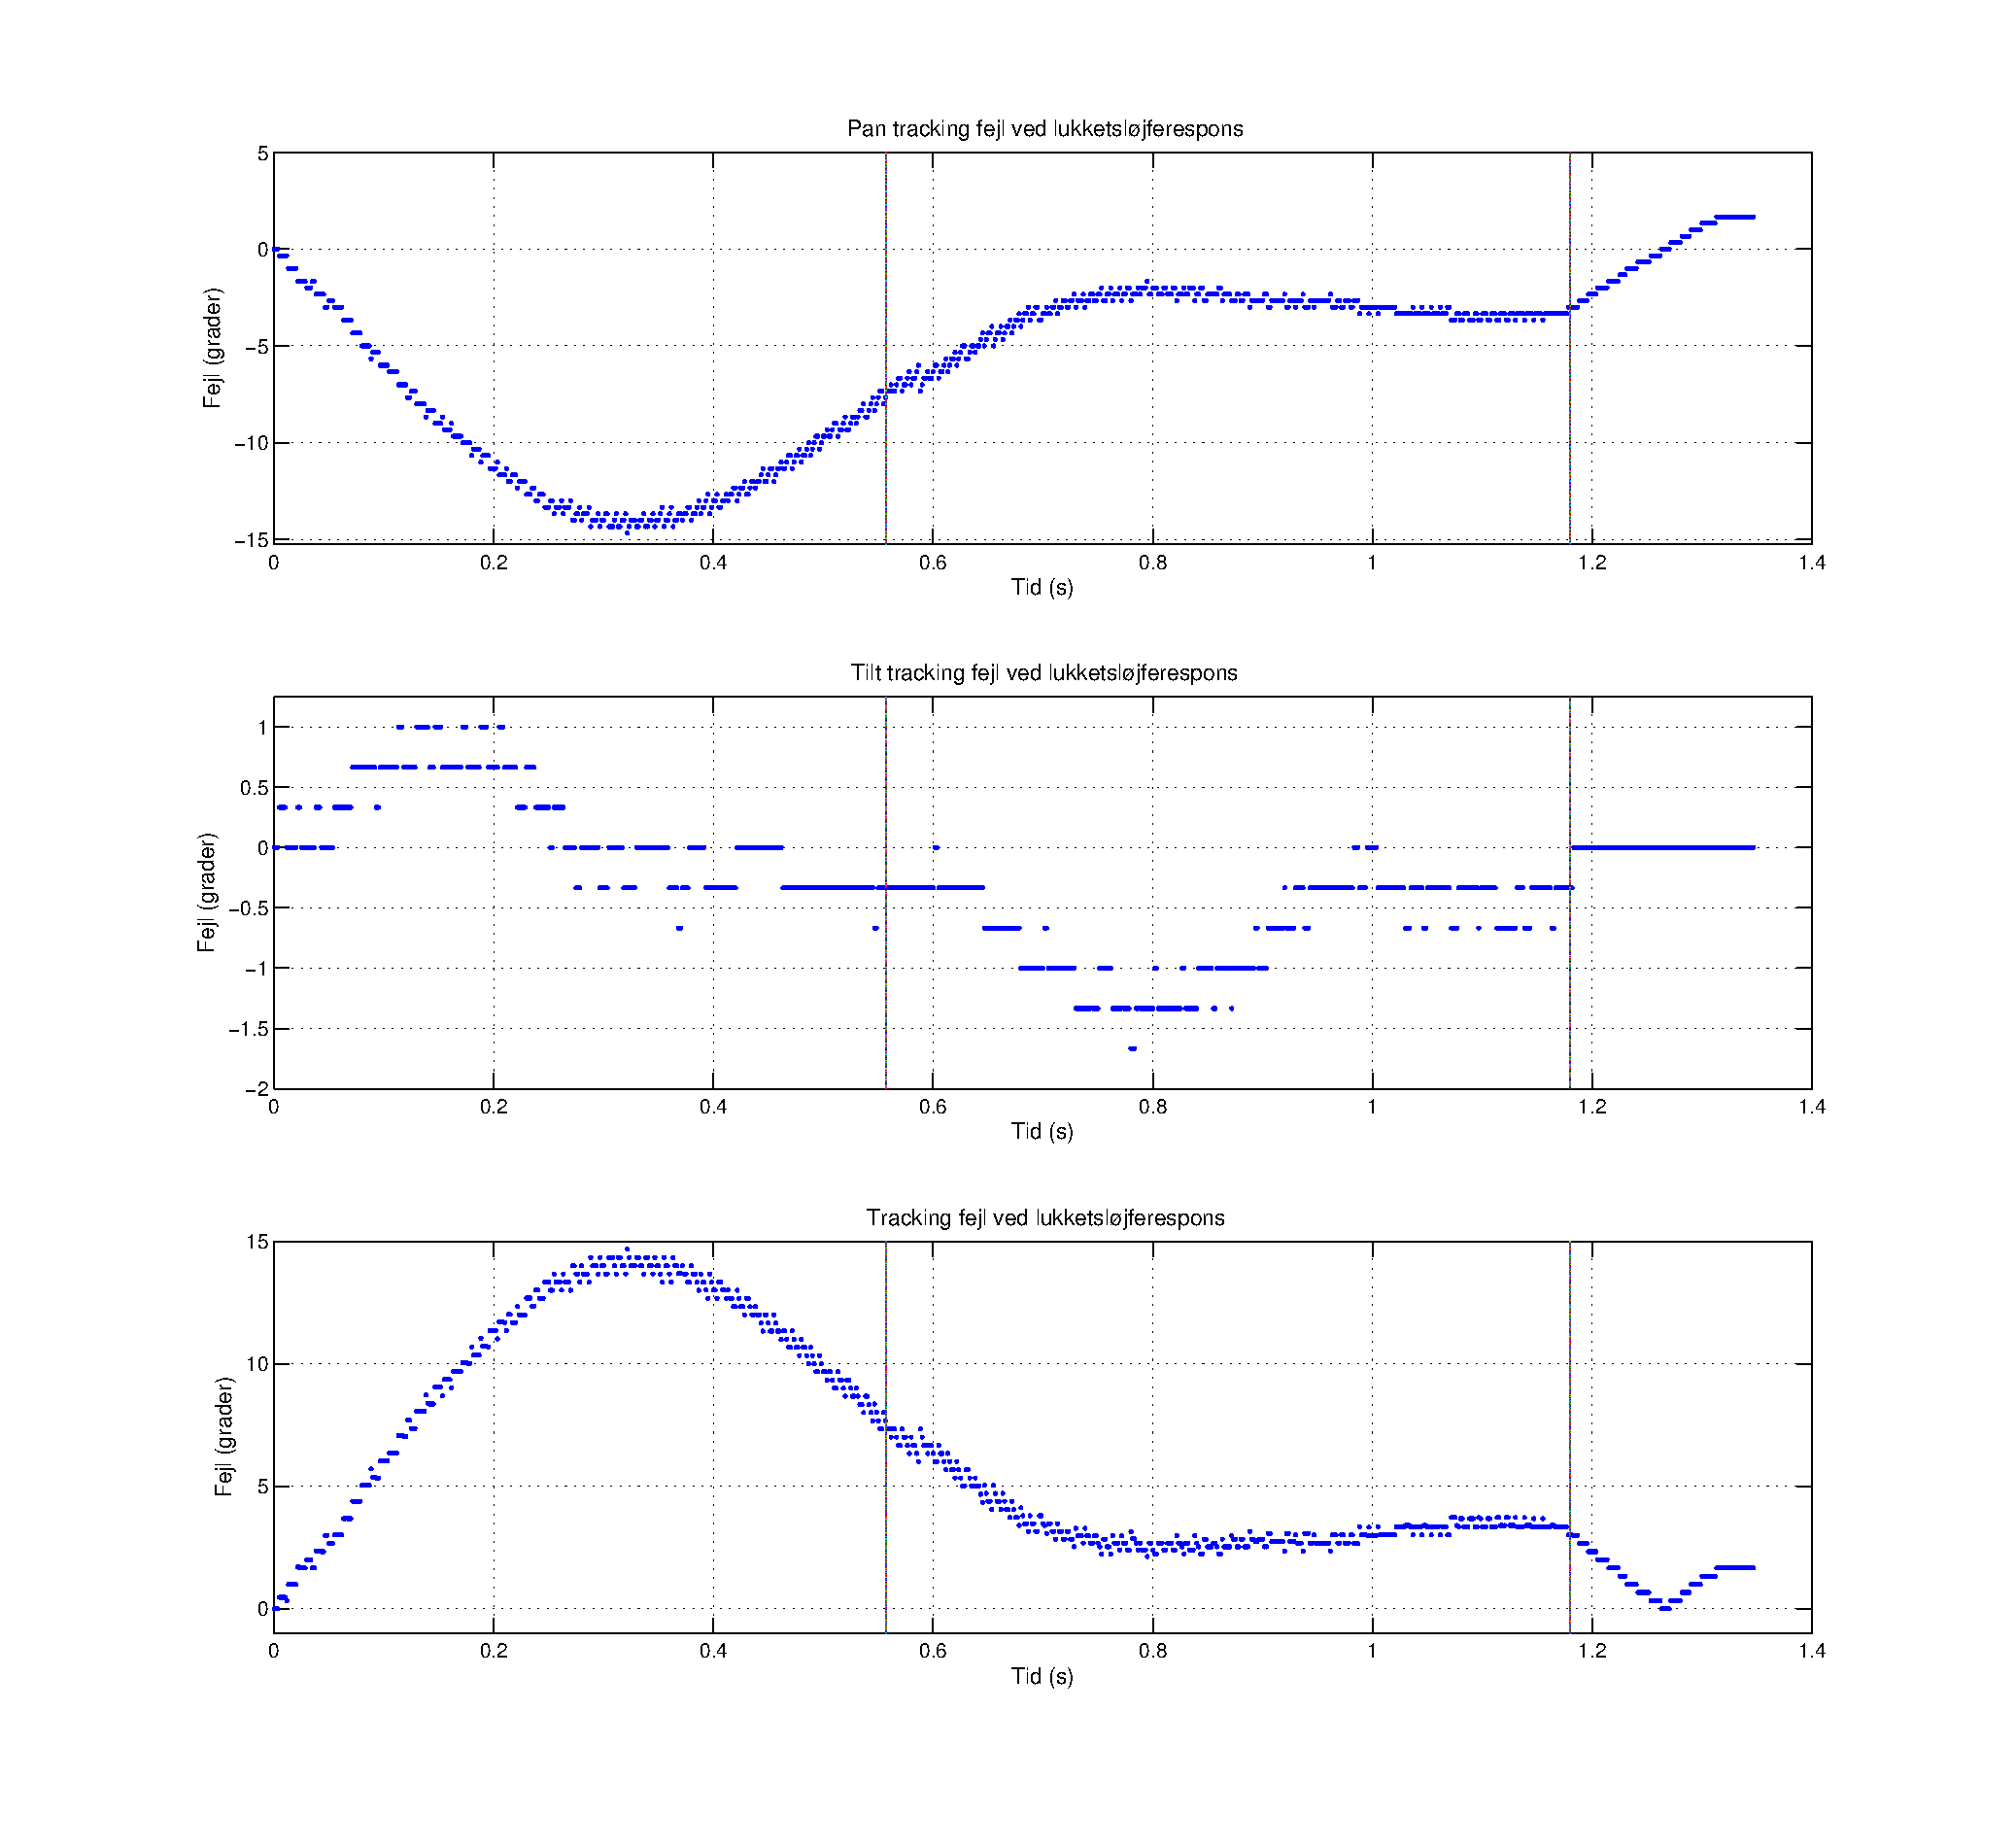
\includegraphics[width=1\textwidth]{./graphics/error_start.eps}
\caption[Regulator koefficienter brugt i test]{Tracking fejl målt i grader for hhv. pan og tilt samt den samlet tracking fejl. Testen tager udgangspunkt i koefficienterne fra  tabel \ref{tb:PID_test14}.} 
\label{fig:PID_test14_plot}
\end{figure}

\subsection{Optimering af controllerkoefficienter}
Som det fremgår af figur \ref{fig:PID_test14_plot}, er den samlet tracking fejl XXXXXXXXXXXXXX i forhold til kravene for PTS. Grundet tracking fejlen skal optimeringen af controller koefficienterne foretages manuelt.

Finjusteringen af controller koefficienterne udføres som en iterativ proces. Optimeringsprocessen er opdelt i to, således der kun foretages ændringer for enten pan eller tilt. 
Optimerings iterationerne tager udgangspunkt i en grafisk afbildning af tracking fejlen, hvor efter det vurderes hvorledes hver controller koefficient skal øges eller mindskes for at få det ønsket resultat. 

Der blev foretaget XXXXXXXXXX ilterationer og det lykkes at få en samlet tracking fejl som opfylder kravet, angivet i ligning \ref{eq:ks:trackingerror}.



\subsection{PTS verifikation}



For ilteration XXXXXXXXX med controller koefficienterne angivet i tabel \ref{tb:PID_final}, er det lykkedes at opfylde kravet om den samlede tracking fejl som stilles for PTS. 
Figur \ref{fig:PID_final} viser tracking fejlen for hhv. pan og tilt samt den samlede tracking fejl. 
\begin{figure}[h!]
\centering
\begin{tabu}{l|[1.25pt]c|c|c}
      & \(K_P\) & \(K_I\) & \(K_D\)\\\tabucline[1.25pt]{-}
Tilt  &  &  & \\\hline
Pan   & & &
\end{tabu}
\captionsetup{type=table}
\caption[Endelig regulator koefficienter]{Angivet koefficienter opfylder kravet til PTS.}
\label{tb:PID_final} 
\end{figure}







\begin{figure}[h!]
\centering
%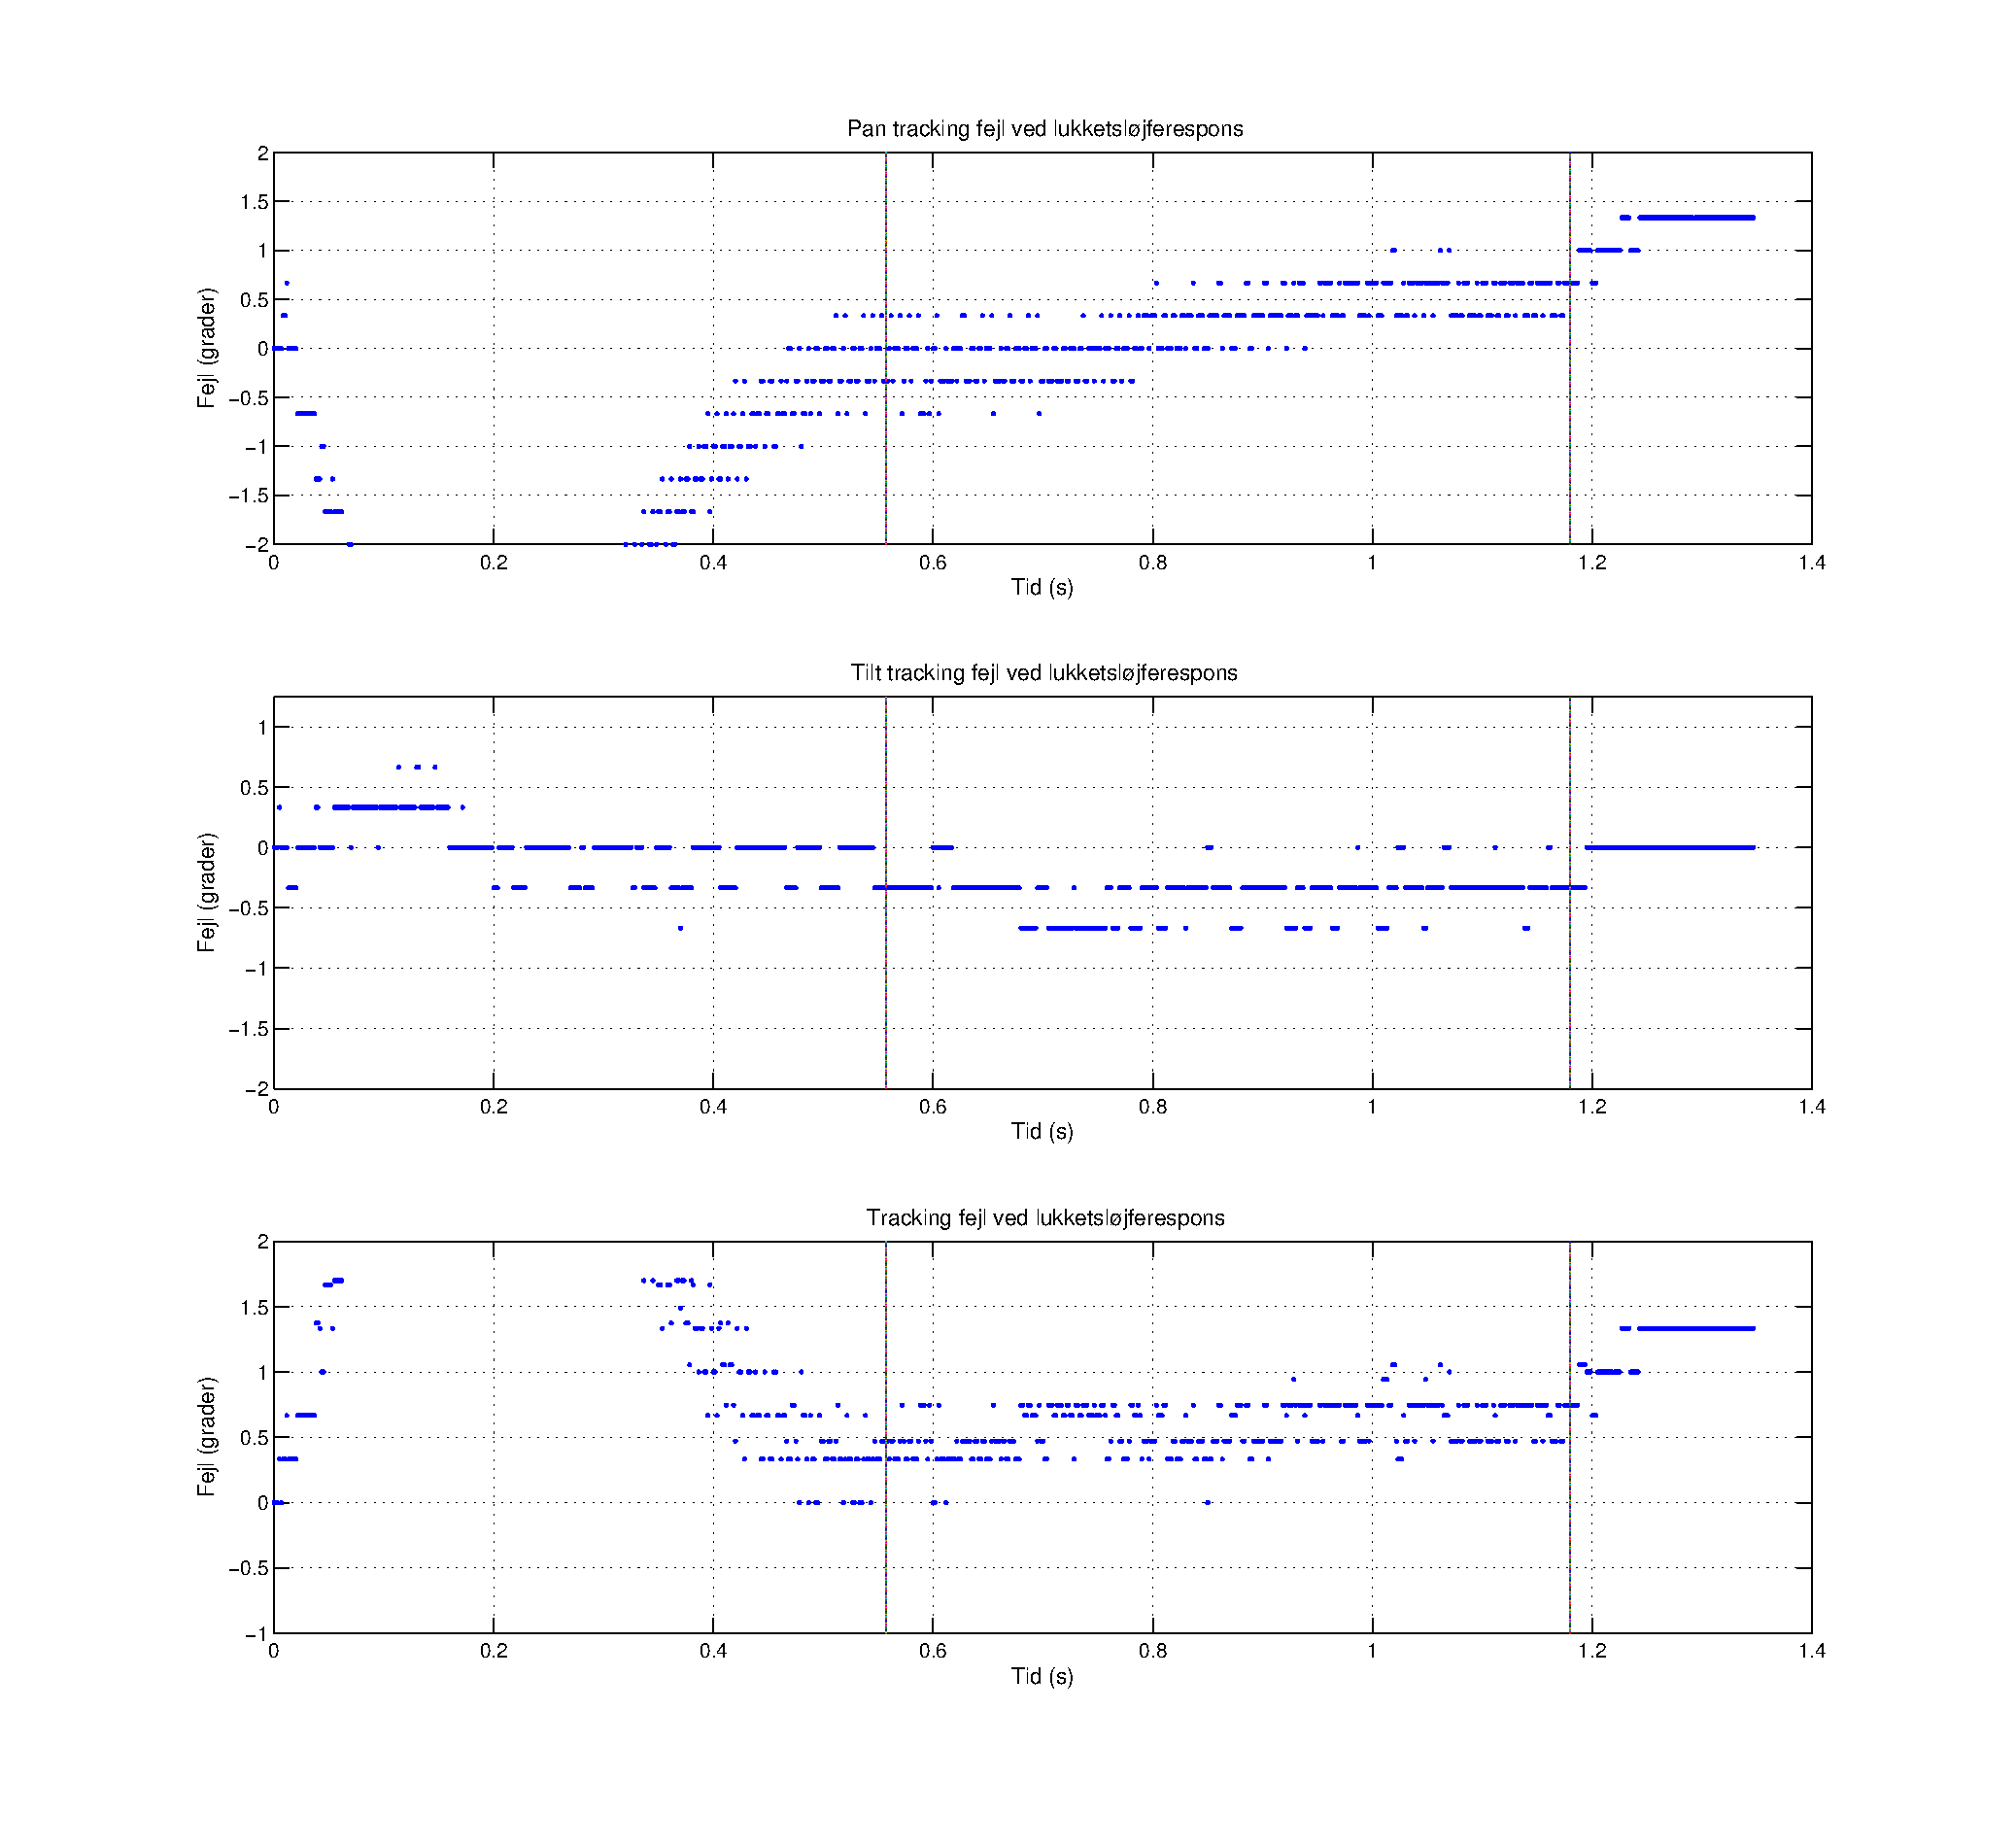
\includegraphics[width=1\textwidth]{./graphics/error_slut.eps}
\caption[Endelig regulator koefficienter]{Tracking fejl målt i grader for hhv. pan og tilt samt den samlet tracking fejl. Testen tager udgangspunkt i koefficienterne fra  tabel \ref{tb:PID_final} og det ses at den samlet tracking fejl opfylder kravet til PTS.} 
\label{fig:PID_final}
\end{figure}